\documentclass[10pt,a4paper,final]{article}
\usepackage[utf8]{inputenc}
\usepackage[T1]{fontenc}
\usepackage{lmodern}
\usepackage[margin=2.5cm]{geometry}
\usepackage{amsmath}
\usepackage{amssymb}
\usepackage{mathtools}
\usepackage{microtype}
\usepackage{float}
\usepackage{xcolor}
\usepackage[affil-it]{authblk}
\usepackage{booktabs}
\usepackage{tabularx}
\usepackage{enumitem}
\usepackage{bytefield}
\usepackage{tikz}
\usetikzlibrary{arrows.meta,positioning,fit,calc,shapes.geometric,backgrounds}
\usepackage[pdftex,
    pdfauthor={Adam Waldenberg, The Unigrid Foundation},
    pdftitle={Sharded and redundant storage on the Unigrid Network},
    pdfsubject={White Paper},
    pdfkeywords={unigrid;hedgehog;gridnode;storage;erasure coding;reed-solomon;encryption;sharding;decentralized}]{hyperref}

\let\oldhref\href
\renewcommand{\href}[2]{\oldhref{#1}{\bfseries#2}}
\hypersetup{colorlinks = true, urlcolor = black, citecolor = black, linkcolor = black}
\author{\textit{Adam Waldenberg\\\href{mailto:adam@unigrid.org}{adam@unigrid.org}}}
\affil{The Unigrid Foundation\\\href{http://www.unigrid.org}{www.unigrid.org}}
\title{Sharded and redundant storage on the Unigrid Network}
\date{\emph{Draft version (\today)}}

\newcommand{\code}[1]{\texttt{#1}}
\newcommand{\cat}{\mathbin{\|}}
\newcolumntype{L}{>{\raggedright\arraybackslash}X}
\setlist{itemsep=2pt, topsep=4pt}

\tikzset{
	stage/.style={draw, rounded corners=3pt, align=left, text width=3.9cm, inner sep=6pt, font=\small},
	zone/.style={draw, rounded corners=4pt, inner sep=8pt},
	flow/.style={-{Stealth[length=2.2mm]}, thick},
	cell/.style={draw, minimum width=5mm, minimum height=5mm, inner sep=0pt, font=\scriptsize},
	decision/.style={draw, diamond, aspect=2.2, align=center, inner sep=1pt, font=\small},
	action/.style={draw, rounded corners=3pt, align=center, text width=3.4cm, inner sep=5pt, font=\small}
}

\begin{document}

\maketitle

\begin{abstract}
Hedgehog stores a file on the Unigrid Network as many small, encrypted fragments spread over the active
gridnodes, with enough redundancy that the file survives the loss of a large share of them. One random 256-bit
secret, the \emph{fingerprint}, both locates and decrypts the file, and the network keeps no other record of who
owns it. Two layers of Reed-Solomon erasure coding divide the work. An outer layer, whose structure only the owner
knows, protects the file against lost chunks. An inner layer lets gridnodes verify and rebuild every chunk on
their own, without learning which chunks belong together, so no party except the fingerprint holder ever has the
full picture. The Unigrid Foundation governs every parameter through a signed \emph{StorageSpork}. Each file
records the parameters it was written with, and a format identifier travels with every stored structure, so the
network can evolve without breaking what it already holds.
\end{abstract}

\tableofcontents

\section{Introduction}

Gridnodes provide the Unigrid Network with storage space, communication channels and compute cycles. This paper
describes the storage layer: how a file is cut up, encrypted, coded, placed, found again, repaired and deleted, and
what every participant can and cannot learn along the way. It is a description of the protocol as implemented in
Hedgehog, and every constant in it is the value the implementation uses.

The storage layer is deliberately low level. It stores opaque files and returns a fingerprint; it knows nothing
about names, folders or buckets. An object-storage interface in the style of S3 is planned as a separate layer that
calls this one.

\section{Goals and threat model}

The design has six goals:

\begin{enumerate}
	\item \textbf{Durability.} A file survives gridnode churn and disk loss while its owner is offline, because
	      gridnodes repair lost fragments themselves.
	\item \textbf{Confidentiality.} Only the fingerprint holder can read the file.
	\item \textbf{Unlinkability.} No gridnode, repairer or holder of stored data can tell which fragments form a
	      file, how large the file is, or who uploaded it.
	\item \textbf{Self-verification.} Anyone can check that a fragment is genuine without knowing a secret.
	\item \textbf{Governance.} The foundation tunes the network through one signed spork, and old files never
	      depend on its current values.
	\item \textbf{Evolvability.} A format identifier travels with every structure, so a later format can live
	      beside the current one.
\end{enumerate}

Table~\ref{tab:threats} lists what each party can see or do, and what the design denies it.

\begin{table}[H]
\centering
\small
\begin{tabularx}{\linewidth}{@{}>{\raggedright\arraybackslash}p{2.4cm}LL@{}}
\toprule
Party & Sees or can do & Cannot \\
\midrule
Curious gridnode & Its own fragments, one signed descriptor per fragment, the source and timing of requests &
Read plaintext, learn a file's size or owner, link two groups, or rebuild a chunk alone: it holds at most one
fragment of any group \\
Repairing gridnode & The ciphertext of one chunk and the gridnodes that hold its fragments & Decrypt that chunk or
find the other chunks of the same file \\
Fragment forger & Send made-up or corrupted fragments & Have them stored or used: every fragment is checked
against its group identifier, a signed descriptor and a Merkle proof \\
Lying census peer & Answer repair queries falsely & Delete a group, because a tombstone claim must carry the
owner's signed proof; false claims of holding a fragment are caught by random spot-checks \\
Network observer & Encrypted QUIC traffic and its timing & Read packet contents \\
Fingerprint holder & Find, read and delete the file & --- \\
\bottomrule
\end{tabularx}
\caption{What each party can and cannot learn or do.}
\label{tab:threats}
\end{table}

Out of scope are an attacker that controls most gridnodes, global traffic analysis, and denial of service beyond
what the per-node quotas limit.

\section{Architecture}

A stored file passes through six steps (Figure~\ref{fig:pipeline}). The first three run on the uploader's own
node and produce a structure that only the owner knows. The last three produce material that any gridnode can
check, store and repair.

\begin{figure}[H]
\centering
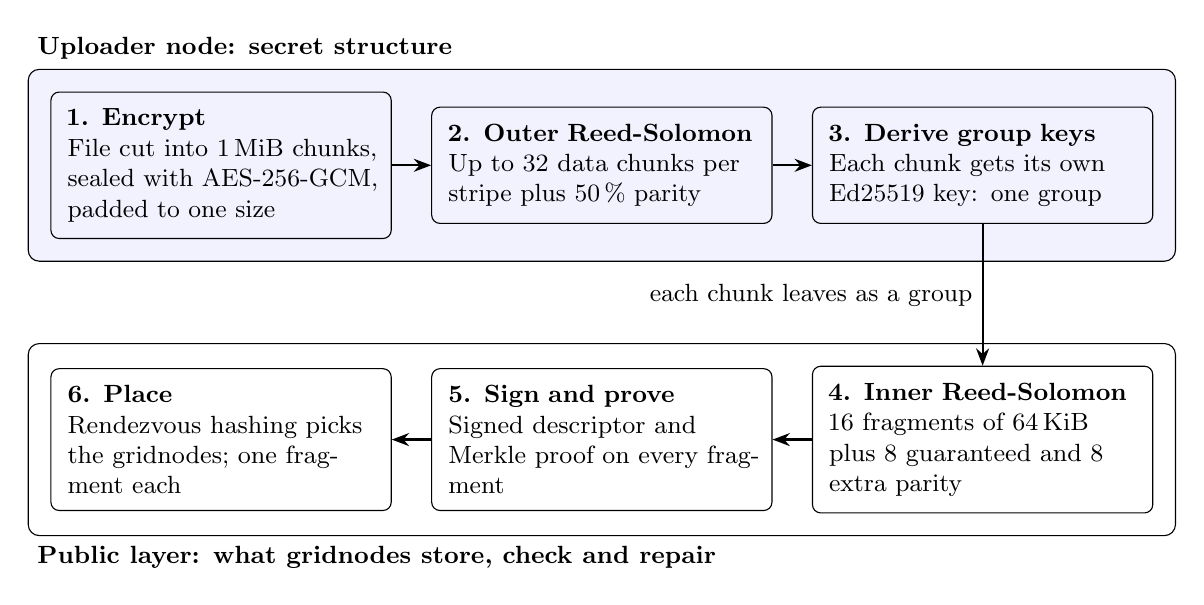
\begin{tikzpicture}[node distance=6mm and 5mm]
	\node[stage] (enc) {\textbf{1. Encrypt}\\File cut into 1\,MiB chunks, sealed with AES-256-GCM, padded to one size};
	\node[stage, right=of enc] (outer) {\textbf{2. Outer Reed-Solomon}\\Up to 32 data chunks per stripe plus 50\,\% parity};
	\node[stage, right=of outer] (keys) {\textbf{3. Derive group keys}\\Each chunk gets its own Ed25519 key: one group};
	\node[stage, below=18mm of keys] (inner) {\textbf{4. Inner Reed-Solomon}\\16 fragments of 64\,KiB plus 8 guaranteed and 8 extra parity};
	\node[stage, left=of inner] (sign) {\textbf{5. Sign and prove}\\Signed descriptor and Merkle proof on every fragment};
	\node[stage, left=of sign] (place) {\textbf{6. Place}\\Rendezvous hashing picks the gridnodes; one fragment each};
	\begin{scope}[on background layer]
		\node[zone, fill=blue!5, fit=(enc)(outer)(keys), label={[font=\small\bfseries, anchor=south west]north west:Uploader node: secret structure}] {};
		\node[zone, fit=(place)(sign)(inner), label={[font=\small\bfseries, anchor=north west]south west:Public layer: what gridnodes store, check and repair}] {};
	\end{scope}
	\draw[flow] (enc) -- (outer);
	\draw[flow] (outer) -- (keys);
	\draw[flow] (keys) -- node[left, font=\small] {each chunk leaves as a group} (inner);
	\draw[flow] (inner) -- (sign);
	\draw[flow] (sign) -- (place);
\end{tikzpicture}
\caption{The storage pipeline at default settings.}
\label{fig:pipeline}
\end{figure}

Four terms recur through this paper:

\begin{description}
	\item[Chunk] A fixed-size piece of ciphertext. Data chunks carry encrypted file bytes; parity chunks come from
	      the outer code.
	\item[Stripe] A run of data chunks together with their outer parity chunks. Only the owner knows which chunks
	      form a stripe.
	\item[Group] One chunk as the network sees it, named by a 32-byte group identifier.
	\item[Fragment] One inner-code piece of a group, the unit a gridnode stores.
\end{description}

The split into two layers is the core of the design. The owner applies the outer code across whole chunks and keeps
the grouping to itself. Gridnodes see only single chunks, each coded again into fragments that they can rebuild on
their own. A repairer therefore holds at most one chunk of ciphertext, and nothing tells it which other chunks
belong to the same file (Figure~\ref{fig:layers}).

\begin{figure}[H]
\centering
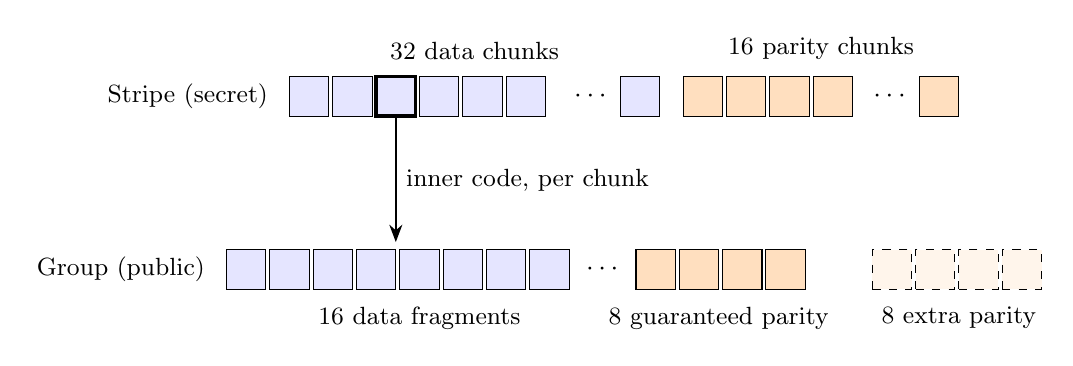
\begin{tikzpicture}
	\foreach \i in {0,...,5} \node[cell, fill=blue!10] at (\i*0.55, 0) {};
	\node at (3.6, 0) {$\cdots$};
	\node[cell, fill=blue!10] (dlast) at (4.2, 0) {};
	\foreach \i in {0,...,3} \node[cell, fill=orange!25] at (5.0+\i*0.55, 0) {};
	\node at (7.4, 0) {$\cdots$};
	\node[cell, fill=orange!25] (plast) at (8.0, 0) {};
	\node[font=\small, anchor=south] at (2.1, 0.35) {32 data chunks};
	\node[font=\small, anchor=south] at (6.5, 0.35) {16 parity chunks};
	\node[font=\small, anchor=east] at (-0.4, 0) {Stripe (secret)};
	\node[cell, fill=blue!10, very thick] (pick) at (1.1, 0) {};
	\foreach \i in {0,...,7} \node[cell, fill=blue!10] at (\i*0.55-0.8, -2.2) {};
	\node at (3.75, -2.2) {$\cdots$};
	\foreach \i in {0,...,3} \node[cell, fill=orange!25] at (4.4+\i*0.55, -2.2) {};
	\foreach \i in {0,...,3} \node[cell, dashed, fill=orange!8] at (7.4+\i*0.55, -2.2) {};
	\node[font=\small, anchor=north] at (1.4, -2.55) {16 data fragments};
	\node[font=\small, anchor=north] at (5.2, -2.55) {8 guaranteed parity};
	\node[font=\small, anchor=north] at (8.25, -2.55) {8 extra parity};
	\node[font=\small, anchor=east] at (-1.2, -2.2) {Group (public)};
	\draw[flow] (pick.south) -- (1.1, -1.85) node[midway, right, font=\small] {inner code, per chunk};
\end{tikzpicture}
\caption{Two-level coding at default settings. The outer code spans a stripe that only the owner can reconstruct;
the inner code spans one chunk and is visible to every gridnode that stores it.}
\label{fig:layers}
\end{figure}

\section{Locating a file}

The fingerprint is the only input retrieval needs. Every address and key the network uses for a file is derived
from it, and nothing else about the file is stored anywhere.

\subsection{The fingerprint}

The secret is 32 bytes from a cryptographically secure random generator, drawn fresh for every upload. Users see it
as Base58Check text: the format identifier as version byte, the secret, and a 4-byte double-SHA-256 checksum. These
37 bytes are written as 50 Base58 characters. Parsing trims the text, verifies the checksum, requires exactly 33
decoded bytes, and requires a known format identifier. A mistyped character fails the checksum, so a typo is
rejected before any network traffic.

\subsection{Derived keys}

Every key comes from HKDF-SHA256 over the secret, with the format-specific salt \code{"hedgehog-storage-v1"} and a
32-byte output:
\begin{equation}
	K_{\mathit{label}} = \mathrm{HKDF\text{-}SHA256}(\mathit{IKM} = \mathit{secret},\ \mathit{salt},\ \mathit{info} = \mathit{label},\ L = 32)
\end{equation}

\begin{table}[H]
\centering
\small
\begin{tabularx}{\linewidth}{@{}p{4.6cm}cL@{}}
\toprule
Info label & Bytes & Used as \\
\midrule
\code{"enc"} & 3 & AES-256 key for every chunk of the file \\
\code{"manifest-enc"} & 12 & AES-256 key for the manifest \\
\code{"manifest"} $\cat$ u8 \textit{copy} & 9 & Ed25519 seed of manifest copy \textit{copy} (0--255) \\
\code{"chunk"} $\cat$ u32 \textit{stripe} $\cat$ u8 \textit{index} & 10 & Ed25519 seed of chunk \textit{index}
(0--255) in stripe \textit{stripe} \\
\bottomrule
\end{tabularx}
\caption{Key-derivation labels.}
\end{table}

\subsection{Group identifiers}

Each seed is used directly as an RFC~8032 Ed25519 private key. The 32-byte public key is hashed to name the group:
\begin{equation}
	\mathit{groupId} = \mathrm{SHA\text{-}256}(\mathit{publicKey})
\end{equation}

Every seed comes from its own HKDF expansion under a distinct label. Without the secret, two group identifiers of
one file are indistinguishable from identifiers of two unrelated files. This is what keeps the network from linking
chunks together.

\subsection{Finding the pieces}

\begin{enumerate}
	\item Derive the manifest group keys and their group identifiers.
	\item Rank the active gridnodes for each identifier (Section~\ref{sec:placement}) and fetch fragments from the
	      top of the ranking.
	\item Decrypt the manifest. It gives the file size and the layout the file was written with.
	\item Derive the identifier of every chunk group from its stripe and index, and fetch those groups the same way.
\end{enumerate}

The manifest search runs in two passes, because the spork may have changed since the upload. The narrow pass looks
for copies 0 to 15, the highest count the spork allows, in the current placement window of 40 gridnodes. The wide
pass looks for the copies the current spork names across $255 + \mathit{slack}$ gridnodes, 263 with the defaults.

A wrong fingerprint and a fully lost file give the same answer: \emph{not found}. This is deliberate. The network
cannot confirm that a guessed fingerprint exists.

\section{Ownership without accounts}

The network keeps no owner record: whoever holds the fingerprint owns the file. There are no accounts, no uploader
signatures and no per-user index. A gridnode sees which Hedgehog node sent it a fragment, but it stores nothing that
ties the fragment to that node. Ownership gives two powers, and both follow from keys derived from the fingerprint:

\begin{itemize}
	\item \textbf{Read.} Only the fingerprint yields the manifest key and the chunk key.
	\item \textbf{Delete.} Only the fingerprint yields the private key of each group, and only that key signs a
	      valid delete.
\end{itemize}

\subsection{The delete proof}

A delete is one \code{DELETE\_GROUP} packet per group, sent to every gridnode in that group's placement window. It
carries the group's public key, a timestamp in epoch milliseconds, and an Ed25519 signature over a 52-byte message:
\begin{equation}
	m = \texttt{"hh-delete-v1"} \cat \mathit{groupId}_{[32]} \cat \mathit{timestamp}_{\mathrm{i64}}
\end{equation}

A gridnode accepts the delete only if the public key hashes to the group identifier and the signature verifies. The
proof is \emph{self-certifying}: it needs no stored state to check. Even a gridnode that does not hold the group can
verify it and keep it as a tombstone.

\begin{table}[H]
\centering
\small
\begin{tabular}{@{}ll@{}}
\toprule
Receiver state & Answer \\
\midrule
No valid StorageSpork & \code{DISABLED} \\
Group already tombstoned & \code{OK} \\
Proof fails & \code{INVALID} \\
Group not held and the tombstone budget is spent & \code{QUOTA} \\
Otherwise: tombstone written, any held fragment removed & \code{OK} \\
\bottomrule
\end{tabular}
\caption{How a gridnode answers a delete.}
\end{table}

A tombstone lives for \code{tombstoneDays}, 30 by default. While it lives, the gridnode refuses new stores of that
group and hands the signed proof to any repairer that asks about it. A holder that missed the delete therefore
learns of it at the next census, verifies the proof, and drops its fragment. A claimed tombstone without a valid
proof is ignored.

\subsection{Consequences}

\begin{itemize}
	\item A lost fingerprint means a lost file. There is no recovery path.
	\item Sharing a fingerprint shares full ownership, delete included. The format has no read-only rights.
	\item Storage is charged to each gridnode's own quota, not to an owner. There is no payment or per-owner limit.
\end{itemize}

\section{Encryption}

Every chunk is AES-256-GCM ciphertext of exactly \code{chunkSize} bytes, so no stored piece reveals content,
position or file size.

\begin{table}[H]
\centering
\small
\begin{tabularx}{\linewidth}{@{}p{2.6cm}LL@{}}
\toprule
Element & Data chunks & Manifest \\
\midrule
Key & HKDF label \code{"enc"} & HKDF label \code{"manifest-enc"} \\
Nonce (12 bytes) & u64 \textit{sequence} $\cat$ u32 0 & u64 \textit{copy} $\cat$ u32 1 \\
Additional data & \code{"hh-chunk-v1"} $\cat$ u64 \textit{sequence} & \code{"hh-manifest-v1"} $\cat$ u64 \textit{copy} \\
Plaintext & File bytes, zero-padded to $\mathit{chunkSize} - 16$ & 26-byte manifest, zero-padded to $\mathit{chunkSize} - 16$ \\
Tag & 16 bytes & 16 bytes \\
\bottomrule
\end{tabularx}
\caption{Authenticated encryption parameters.}
\end{table}

The chunk sequence is a global chunk number, $\mathit{stripe} \cdot \mathit{maxOuterDataChunks} + i$. Each upload
draws a fresh fingerprint and therefore fresh keys, so a nonce never repeats under one key. The domain word keeps
chunk and manifest nonces apart.

\paragraph{Uniform size.} With the defaults a data chunk carries 1\,048\,560 bytes of file data, and the 16-byte
tag fills it to exactly 1\,MiB. The manifest is padded to the same size. A manifest group looks exactly like a data
group, and the last chunk of a file looks like any other.

\paragraph{Tamper resistance.} The sequence number sits in both the nonce and the additional data. A chunk moved to
another position, or taken from another file, fails authentication. The manifest's file size fixes the number of
data chunks, so truncation is detected. Corrupt fragments are usually rejected earlier by their Merkle proof. A
chunk that still fails authentication stops retrieval with a data-loss error, never with wrong output.

\paragraph{Parity.} Outer parity chunks are Reed-Solomon combinations of ciphertext chunks. They are as
indistinguishable from random as the ciphertext they come from and need no further encryption.

\section{Erasure coding}

Both layers use one systematic Cauchy Reed-Solomon code over $\mathrm{GF}(2^8)$: any $k$ of the $k + m$ shards
rebuild the data. The implementation has no external dependency.

\subsection{The field}

Bytes are elements of $\mathrm{GF}(2^8)$ with the reducing polynomial $x^8 + x^4 + x^3 + x^2 + 1$ (\code{0x11D})
and generator 2. Addition is XOR. Multiplication uses a precomputed $256 \times 256$ product table of 64\,KiB beside
the usual exponent and logarithm tables, and the inverse is $\mathrm{EXP}[255 - \mathrm{LOG}[a]]$.

\subsection{The encoding matrix}

The $k$ data shards pass through unchanged. Parity row $r$, for $0 \le r < m$, combines them with a Cauchy matrix:
\begin{equation}
	p_r = \bigoplus_{c=0}^{k-1} C_{r,c} \cdot d_c, \qquad C_{r,c} = \frac{1}{(k + r) \oplus c}
\end{equation}

The row values $k, \dots, k+m-1$ and the column values $0, \dots, k-1$ never overlap. Every square submatrix of a
Cauchy matrix is then invertible, which makes the code maximum-distance separable: \emph{any} $k$ shards suffice. A
code has at most 255 shards.

\paragraph{Prefix property.} A parity row depends only on its absolute position $k + r$, never on $m$. The parity of
$\mathrm{RS}(k, m_1)$ is therefore the first $m_1$ rows of $\mathrm{RS}(k, m_2)$. The inner layer relies on this:
each chunk is encoded once to $n_{max}$ fragments. Fragments $0$ to $n_{in} - 1$ are exactly the guaranteed code,
and the rest are extra parity that gridnodes may keep or drop.

\subsection{Worked example}

Take $k = 2$ and $m = 1$. The single parity row is $C = (1/2,\ 1/3)$. In this field $1/2 = \mathtt{0x8E}$ and
$1/3 = \mathtt{0xF4}$, so each parity byte is
\begin{equation}
	p = \mathtt{0x8E} \cdot d_0 \oplus \mathtt{0xF4} \cdot d_1 .
\end{equation}
If $d_0$ is lost, one multiplication by 2, the inverse of \code{0x8E}, restores it:
\begin{equation}
	d_0 = 2 \cdot (p \oplus \mathtt{0xF4} \cdot d_1) .
\end{equation}

\subsection{Decoding}

The decoder takes the first $k$ present shards, builds their $k \times k$ submatrix and inverts it by Gauss-Jordan
elimination over $\mathrm{GF}(2^8)$ in $O(k^3)$. It multiplies the inverse by the shards to recover the data in
$O(k^2 L)$ for shard length $L$, and re-encodes any missing parity. Retrieval skips the outer decode when every data
chunk arrived.

\subsection{Layout}
\label{sec:layout}

With $\mathrm{pct}(v, p) = \lceil v \cdot p / 100 \rceil$, a file of $\mathit{fileSize}$ bytes is laid out as
follows:
\begin{align}
	\mathit{payload} &= \mathit{chunkSize} - 16 & D &= \max\left(1, \left\lceil \mathit{fileSize} / \mathit{payload} \right\rceil\right) \\
	S &= \left\lceil D / \mathit{maxOuterDataChunks} \right\rceil & k_s &= \min(\mathit{maxOuterDataChunks},\ D - s \cdot \mathit{maxOuterDataChunks}) \\
	m_s &= \mathrm{pct}(k_s, \mathit{outerParity}) & k_{in} &= \mathit{chunkSize} / \mathit{fragmentSize} \\
	m_{in} &= \mathrm{pct}(k_{in}, \mathit{innerParity}) & n_{in} &= k_{in} + m_{in} \\
	n_{max} &= k_{in} + \mathrm{pct}(k_{in}, \mathit{maxParity}) & W &= n_{max} + \mathit{placementSlack}
\end{align}

\begin{table}[H]
\centering
\small
\begin{tabularx}{\linewidth}{@{}lcL@{}}
\toprule
Quantity & Default & Meaning \\
\midrule
$k_{in}$ / $m_{in}$ / $n_{in}$ & 16 / 8 / 24 & Guaranteed fragments per chunk; any 16 rebuild it \\
$n_{max}$ & 32 & Fragment slots per chunk, extras included \\
$W$ & 40 & Gridnodes in a group's placement and search window \\
$k_s$ / $m_s$ & up to 32 / 16 & Data and parity chunks of a full stripe; any 32 of 48 rebuild it \\
\bottomrule
\end{tabularx}
\caption{Code parameters at default settings.}
\end{table}

\subsection{How the layers combine}

A group is lost only when more than 8 of its 24 guaranteed fragments are gone, or more than 16 of 32 when all extras
are held. A lost group is one erasure for the outer code, and a full stripe is lost only when more than 16 of its 48
groups are lost. Table~\ref{tab:loss} assumes that every fragment is lost independently with probability $q$ and
that no repair runs in between.

\begin{table}[H]
\centering
\small
\begin{tabular}{@{}cccc@{}}
\toprule
Fragment loss $q$ & Group lost (24 held) & Group lost (32 held) & Full stripe lost (24 held) \\
\midrule
5\,\% & $1.3 \times 10^{-6}$ & $2.1 \times 10^{-14}$ & $2.9 \times 10^{-88}$ \\
10\,\% & $3.2 \times 10^{-4}$ & $1.3 \times 10^{-9}$ & $1.7 \times 10^{-47}$ \\
20\,\% & $3.6 \times 10^{-2}$ & $3.3 \times 10^{-5}$ & $4.5 \times 10^{-13}$ \\
30\,\% & $0.28$ & $5.2 \times 10^{-3}$ & $0.14$ \\
\bottomrule
\end{tabular}
\caption{Loss probabilities from the binomial distribution under independent fragment loss.}
\label{tab:loss}
\end{table}

These numbers follow from the independence assumption, not from field data. They show that the two layers multiply
their protection, that repair must act well before a third of the fragments are gone, and that held extras push that
point much further.

\section{Storage overhead}

At default settings a large file costs 2.27 times its size across the network. Small files cost far more, because
every file carries three manifest groups and at least one data and one parity chunk.

Each group stores 24 guaranteed fragments of 64\,KiB, 1.5 times the chunk. Each fragment also carries 302 bytes of
proof material: the 136-byte descriptor, 2 bytes of index and proof length, a 160-byte Merkle proof and a 4-byte
length. A file needs $D + \sum_s m_s + \mathit{manifestCopies}$ groups.

\begin{table}[H]
\centering
\small
\begin{tabular}{@{}rrrrrrr@{}}
\toprule
File & Data chunks & Outer parity & Groups & Fragments & Stored bytes & Stored / file \\
\midrule
1\,KiB & 1 & 1 & 5 & 120 & 7\,900\,560 & 7\,715$\times$ \\
1\,MiB & 2 & 1 & 6 & 144 & 9\,480\,672 & 9.04$\times$ \\
32\,MiB & 33 & 17 & 53 & 1\,272 & 83\,745\,936 & 2.50$\times$ \\
1\,GiB & 1\,025 & 513 & 1\,541 & 36\,984 & 2\,434\,952\,592 & 2.27$\times$ \\
\bottomrule
\end{tabular}
\caption{Network-wide cost of guaranteed fragments with their proof material, as quotas charge it. On disk each
fragment adds a 12-byte header.}
\end{table}

A 1\,MiB file needs two data chunks, because each chunk holds 16 bytes less than 1\,MiB to leave room for the
authentication tag. For large files the outer and inner parity each add 50\,\%, which approaches
$1.5 \times 1.5 = 2.25$ plus 0.46\,\% of proof material. When gridnodes also keep all extras the network holds up to a
third more, 3\,246\,603\,456 bytes for the 1\,GiB file, but extras only ever use idle quota.

\section{Manifest and format versioning}

\subsection{The manifest}

The manifest is 26 bytes of plaintext, padded and encrypted to one full chunk (Figure~\ref{fig:manifest}). It is
stored \code{manifestCopies} times, 3 by default and at most 16. Each copy is an independent group with its own key,
placed on its own gridnodes. Retrieval accepts a manifest only if it decrypts, its layout is valid, and its format
matches the fingerprint's.

\begin{figure}[H]
\centering
\begin{bytefield}[bitwidth=0.08\linewidth]{10}
	\bitheader{0-9} \\
	\bitbox{1}{\scriptsize fmt} & \bitbox{8}{fileSize (u64)} & \bitbox{1}{\scriptsize copies} \\
	\bitbox{4}{chunkSize (u32)} & \bitbox{4}{fragmentSize (u32)} & \bitbox{2}{\scriptsize outer\,\%} \\
	\bitbox{2}{\scriptsize maxOuter} & \bitbox{2}{\scriptsize inner\,\%} & \bitbox{2}{\scriptsize maxParity\,\%} & \bitbox[]{4}{}
\end{bytefield}
\caption{Manifest plaintext, 26 bytes, big-endian.}
\label{fig:manifest}
\end{figure}

The foundation may change chunk size, parity or window at any time. An old file is still read with the values in
its manifest; only the manifest search itself uses current values, and its two passes cover every copy count the
spork can name.

\subsection{The format identifier}

The storage format identifier, \code{0x01} today, appears in every structure that outlives a request:

\begin{table}[H]
\centering
\small
\begin{tabularx}{\linewidth}{@{}p{5.4cm}L@{}}
\toprule
Place & Effect \\
\midrule
Fingerprint version byte & Hedgehog knows the format before touching the network \\
HKDF salt \code{"hedgehog-storage-v"} + id & Keys of different formats never collide \\
Manifest byte 0 & Must match the fingerprint \\
Descriptor byte 0 and signature domain \code{"hh-group-v"} + id & A descriptor of one format cannot pass as
another \\
Fragment file header byte 0 & A gridnode knows how to read each file on disk \\
Fetch validation & A fragment of another format counts as missing \\
\bottomrule
\end{tabularx}
\caption{Where the format identifier is stored.}
\end{table}

A gridnode that finds a fragment file of an unknown format at startup leaves it on disk, untouched and uncounted, so
an upgraded node can pick it up. The delete message context and the tombstone file carry no format byte yet; both
have fixed, versioned layouts to which a later format can add one.

\section{Verifiable fragments}

Every fragment carries everything needed to check it, so any gridnode can reject forged or corrupt data without a
secret.

\subsection{The group descriptor}

The uploader signs a 136-byte descriptor for each group with the group's private key (Figure~\ref{fig:descriptor}).
The signature covers the ASCII domain \code{"hh-group-v1"} followed by the first 72 descriptor bytes, an 83-byte
message.

\begin{figure}[H]
\centering
\begin{bytefield}[bitwidth=0.1\linewidth]{8}
	\bitheader{0-7} \\
	\bitbox{1}{\scriptsize fmt} & \bitbox{1}{$k_{in}$} & \bitbox{1}{$m_{in}$} & \bitbox{1}{$n_{max}$} & \bitbox{4}{fragmentSize (u32)} \\
	\wordbox{1}{Ed25519 public key (32 bytes)} \\
	\wordbox{1}{Merkle root (32 bytes)} \\
	\wordbox{1}{Ed25519 signature (64 bytes)}
\end{bytefield}
\caption{Group descriptor, 136 bytes. Each full-width row stands for the field size it names.}
\label{fig:descriptor}
\end{figure}

\subsection{The Merkle tree}

The root commits to all $n_{max}$ fragment slots, extras included. Leaves are padded to a power of two, so the tree
has depth $\lceil \log_2 n_{max} \rceil$: 5 with the defaults and at most 8. Distinct tags separate the three kinds
of node:
\begin{align}
	\mathit{leaf}_i &= \mathrm{SHA\text{-}256}(\mathtt{0x00} \cat \mathrm{u8}\ i \cat \mathit{data}_i) \\
	\mathit{node} &= \mathrm{SHA\text{-}256}(\mathtt{0x01} \cat \mathit{left} \cat \mathit{right}) \\
	\mathit{empty} &= \mathrm{SHA\text{-}256}(\mathtt{0x02})
\end{align}

\subsection{The fragment}

A fragment on the wire is the descriptor, its index, the sibling hashes from leaf to root, and the data:
\begin{multline}
	\mathit{descriptor}_{[136]} \cat \mathrm{u8}\ \mathit{index} \cat \mathrm{u8}\ \mathit{proofLen} \\
	\cat \mathit{proof}_{[32 \cdot \mathit{proofLen}]} \cat \mathrm{u32}\ \mathit{dataLen} \cat \mathit{data}
\end{multline}
With the defaults that is 65\,838 bytes, of which 302 are overhead. A receiver checks, in order:

\begin{enumerate}
	\item the descriptor is well formed: $1 \le k_{in}$, $k_{in} + m_{in} \le n_{max} \le 255$, positive fragment size;
	\item $\mathrm{SHA\text{-}256}(\mathit{publicKey})$ equals the group identifier it expects;
	\item the data length equals the descriptor's fragment size;
	\item the descriptor signature verifies;
	\item the Merkle proof leads from the fragment to the signed root.
\end{enumerate}

A group therefore cannot be forged without its private key, and any altered byte is detected by anyone.

\section{Placement}
\label{sec:placement}

Fragments go to active gridnodes chosen by rendezvous hashing, so any node can compute where a group lives without a
directory service.

\begin{enumerate}
	\item Score every active gridnode as $\mathrm{SHA\text{-}256}(\mathit{groupId} \cat \mathit{gridnodeId})$ and sort
	      the scores in descending order, breaking ties by gridnode identifier. The first $W$ entries form the
	      group's window.
	\item Guaranteed fragment $i$ goes to window rank $i$, for $i < n_{in}$.
	\item Ranks $n_{in}$ to $W - 1$ are spares. When a guaranteed store fails, for any reason, the next spare is
	      tried.
	\item Extra fragments go to remaining spares without waiting for an answer.
\end{enumerate}

A gridnode holds at most one fragment of any group; it answers \code{DUPLICATE} to a second one. When gridnodes join
or leave, rendezvous hashing moves only the fragments whose rank actually changed. A holder that drops out of the
window moves its fragment back inside it (Section~\ref{sec:repair}). The uploader's own node is a gridnode like any
other and serves its own share in-process rather than over the network.

\section{Network protocol}

Storage traffic uses Hedgehog's existing peer-to-peer transport: Netty over QUIC, which encrypts every connection.
Each message starts with an 8-byte frame header (Figure~\ref{fig:frame}). Payloads are limited to 256\,MiB.

\begin{figure}[H]
\centering
\begin{bytefield}[bitwidth=0.1\linewidth]{8}
	\bitheader{0-7} \\
	\bitbox{2}{magic \code{0xBABE}} & \bitbox{2}{type (u16)} & \bitbox{4}{payload length (u32)}
\end{bytefield}
\caption{Frame header.}
\label{fig:frame}
\end{figure}

\subsection{Packets}

Every storage payload starts with a 64-bit request identifier. The identifiers start at a random value and count up.
A reply completes a request only if it arrives on the same connection and has the expected type, and every request
times out after 10 seconds.

\begin{table}[H]
\centering
\small
\begin{tabularx}{\linewidth}{@{}lrLr@{}}
\toprule
Packet & Type & Payload after the request identifier & Size \\
\midrule
\code{STORE\_FRAGMENT} & 3000 & u32 length, encoded fragment & 65\,850 \\
\code{FETCH\_FRAGMENT} & 3010 & group identifier & 40 \\
\code{FRAGMENT\_REPLY} & 3020 & u8 status, u32 length, fragment (empty unless \code{OK}) & $13 + \mathit{len}$ \\
\code{HAS\_FRAGMENT} & 3030 & u16 count ($\le 4096$), group identifiers & $10 + 32n$ \\
\code{FRAGMENT\_STATUS} & 3040 & u16 count ($\le 4096$), entries of group identifier, u8 state, u8 index; a
\code{TOMBSTONE} entry adds public key, timestamp and signature & $10 + 34n$, $+104$ per tombstone \\
\code{DELETE\_GROUP} & 3050 & group identifier, length-prefixed public key, i64 timestamp, length-prefixed
signature & 152 \\
\code{STORAGE\_ACK} & 3060 & u8 status & 9 \\
\bottomrule
\end{tabularx}
\caption{Storage packets. Sizes are payload bytes with default settings, excluding the frame header.}
\end{table}

Fragment states are \code{NONE} (0), \code{HELD} (1) and \code{TOMBSTONE} (2). Status bytes are \code{OK} (0),
\code{QUOTA} (1), \code{INVALID} (2), \code{TOMBSTONE} (3), \code{DISABLED} (4), \code{NOT\_FOUND} (5),
\code{DUPLICATE} (6) and \code{ERROR} (7). A decoder rejects counts above 4096, lengths above 256\,MiB and key or
signature fields of the wrong size before allocating memory.

\subsection{Threading}

Replies arrive on Netty event loops, so the operations that wait for replies never run on one. Uploads, downloads
and deletes run on the REST server's worker threads, and repair runs on its own thread.

\section{Store, retrieve and delete}

\subsection{Store}

\begin{enumerate}
	\item Require a valid StorageSpork and at least $n_{in}$ active gridnodes; otherwise fail before sending anything.
	\item Draw a fresh fingerprint.
	\item Read the input one stripe at a time, so memory stays bounded to one stripe. An empty file becomes one
	      padded chunk.
	\item Encrypt the data chunks of the stripe and compute its outer parity chunks.
	\item Place the stripe's groups one by one, in an order shuffled with a secure random generator. For each group:
	      encode it to $n_{max}$ fragments, build its Merkle tree, sign its descriptor, and send its guaranteed
	      fragments in shuffled order, each delayed by a random 0 to 25\,ms. Wait for every answer and retry refusals
	      on spares. A group fails when fewer than $n_{in}$ gridnodes accept it.
	\item After the last stripe, store the manifest copies as ordinary groups.
	\item On any failure, send \code{DELETE\_GROUP} for every group already placed, then report the error.
\end{enumerate}

\subsection{Retrieve}

\begin{enumerate}
	\item Find a manifest with the two-pass search.
	\item For each group, ask the $k_{in} + 2$ top-ranked gridnodes of its window in parallel, 18 with the defaults.
	      If fewer than $k_{in}$ verified fragments with distinct indices arrive, ask the rest of the window.
	\item Decode each group with the inner code. Fetch a stripe's parity groups only when a data group is missing,
	      and rebuild the missing chunks with the outer code.
	\item Decrypt, write out, and cut the output to the file size.
\end{enumerate}

The first stripe is recovered in full before any output starts. A file whose beginning is lost is therefore reported
as lost at once, not after a partial transfer.

\subsection{Delete}

Delete needs only the manifest, so even a file with lost data can be deleted. For every data, parity and manifest
group it sends a signed \code{DELETE\_GROUP} to the whole window and collects the answers.

\subsection{Interfaces}

The node exposes storage over its local REST interface and the command line.

\begin{table}[H]
\centering
\small
\begin{tabularx}{\linewidth}{@{}p{2.8cm}L@{}}
\toprule
Request & Behaviour \\
\midrule
\code{POST /storage} & Octet-stream body with a required \code{Content-Length} of at most 64\,GiB; answers 201
with the fingerprint, 411 without a length, 413 above the cap \\
\code{GET /storage} & Fingerprint in the \code{X-Fingerprint} header; answers 200 with \code{X-File-Size} and a
streamed body, 404 when not found, 410 when the first stripe is lost \\
\code{DELETE /storage} & Fingerprint in the \code{X-Fingerprint} header; answers 204 \\
Any & 400 for a malformed fingerprint, 503 without a spork or with too few gridnodes \\
\bottomrule
\end{tabularx}
\caption{REST interface.}
\end{table}

The fingerprint travels in a header and never in a path, so it does not end up in access logs. Error answers and log
lines never contain it. On the command line, \code{storage-put} prints the fingerprint; \code{storage-get} writes to a
temporary file and moves it into place only when its length matches \code{X-File-Size}; \code{storage-delete}
removes the file. Both commands that take a fingerprint prompt for it without echo when it is not given.

\section{Self-healing}
\label{sec:repair}

Gridnodes keep every group at full strength without the owner and without learning anything beyond single chunks.

\subsection{Scheduling}

Time is divided into epochs of \code{repairIntervalMinutes}, 60 by default: $e = \lfloor t / \mathit{interval}
\rfloor$. A gridnode starts repairing only once two epoch boundaries have passed since it started, which leaves at
least one full interval for the network to settle. In each epoch exactly one rank of a group's window is on duty:
\begin{equation}
	\mathit{duty}(g, e) = \left(e + \mathit{prefix}_{32}(g)\right) \bmod \left(n_{max}(g) + \mathit{placementSlack}\right)
\end{equation}
where $\mathit{prefix}_{32}(g)$ is the first four bytes of the group identifier as an unsigned integer. The
holder at that rank does the work. This spreads the cost evenly and keeps each group to one census per epoch instead
of one per holder.

\subsection{A duty visit}

Figure~\ref{fig:repair} shows the steps the gridnode on duty takes for one group.

\begin{figure}[htbp]
\centering
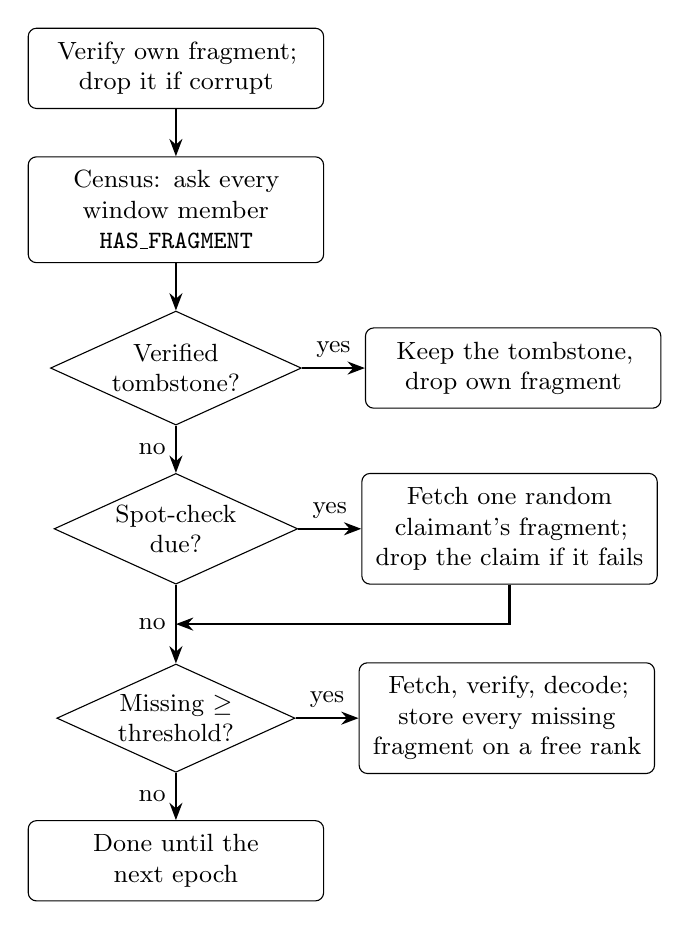
\begin{tikzpicture}[node distance=6mm and 8mm]
	\node[action] (scrub) {Verify own fragment; drop it if corrupt};
	\node[action, below=of scrub] (census) {Census: ask every window member \code{HAS\_FRAGMENT}};
	\node[decision, below=of census] (tomb) {Verified\\tombstone?};
	\node[action, right=of tomb] (delete) {Keep the tombstone, drop own fragment};
	\node[decision, below=of tomb] (spot) {Spot-check\\due?};
	\node[action, right=of spot] (check) {Fetch one random claimant's fragment; drop the claim if it fails};
	\node[decision, below=10mm of spot] (thr) {Missing $\ge$\\threshold?};
	\node[action, right=of thr] (rebuild) {Fetch, verify, decode; store every missing fragment on a free rank};
	\node[action, below=of thr] (done) {Done until the next epoch};
	\draw[flow] (scrub) -- (census);
	\draw[flow] (census) -- (tomb);
	\draw[flow] (tomb) -- node[above, font=\small] {yes} (delete);
	\draw[flow] (tomb) -- node[left, font=\small] {no} (spot);
	\draw[flow] (spot) -- node[above, font=\small] {yes} (check);
	\draw[flow] (check) |- ($(spot.south)!0.5!(thr.north)$);
	\draw[flow] (spot) -- node[left, font=\small] {no} (thr);
	\draw[flow] (thr) -- node[above, font=\small] {yes} (rebuild);
	\draw[flow] (thr) -- node[left, font=\small] {no} (done);
\end{tikzpicture}
\caption{What the gridnode on duty does for one group.}
\label{fig:repair}
\end{figure}

\paragraph{Census.} The census asks every other member of the window whether it holds the group. A \code{HELD}
answer counts only with an index inside the group's slots. A \code{TOMBSTONE} answer counts only when its delete
proof verifies and its public key equals the key in the local descriptor. Every other answer, and silence, counts as
nothing.

\paragraph{Lazy threshold.} Repair costs bandwidth, so it starts only when losses pass a share of the parity budget:
\begin{equation}
	n_{in} - \mathit{present} \ \ge\ \max\left(1,\ \left\lceil m_{in} \cdot \mathit{repairThresholdPercent} / 100 \right\rceil\right)
\end{equation}
where $\mathit{present}$ counts distinct indices, extras included. With the defaults a group is repaired once 4 of
its 24 guaranteed fragments are missing.

\paragraph{Rebuild.} The repairer fetches from every claimant in parallel, keeps only fragments that verify, decodes
the chunk from any $k_{in}$ of them, re-encodes every missing index up to $n_{max}$, and checks that the rebuilt tree
has the signed root. Each rebuilt fragment goes to the next window member that answered \code{NONE}.

\paragraph{Spot-checks.} A gridnode could claim to hold a fragment it has dropped and so delay repair. On every
fourth duty visit to a group, the repairer picks one claimant with a secure random generator and fetches its
fragment. A claim that does not verify is dropped, and repair starts if the group then falls below the threshold.
With $L$ colluding liars, repair is delayed at most until real losses reach $T + L - 1$ for threshold $T$.

\paragraph{Relocation.} A holder whose rank drops out of the window after churn first runs a census, so a deleted
group is never moved. It then offers the fragment to free window members one by one. A member counts only after it
stores the fragment and serves back a verified copy with the same index; only then does the holder remove its own
copy.

\paragraph{Growth limits.} A gridnode accepts fragment sizes between 1/16 and 16 times the current spork value, and
a repairer rebuilds only groups whose full size is at most $\min(\mathit{maxBytesPerNode},\ 16 \cdot n_{max} \cdot
\mathit{fragmentSize})$ under the current spork, 32\,MiB with the defaults. These limits stop old or malicious
descriptors from making gridnodes allocate unbounded memory.

\subsection{What a repairer learns}

During a rebuild the repairer holds the ciphertext of one chunk and knows which gridnodes hold its fragments. It has
no key to decrypt the chunk and no way to find the other chunks of the file, because their group identifiers are
unrelated to this one.

\section{Extra-parity pool and quotas}

Each gridnode's store has two tiers, and idle disk space adds durability without ever displacing guaranteed data.

\begin{description}
	\item[Guaranteed] Fragments with index below $n_{in}$. They may use the whole quota, \code{maxBytesPerNode},
	      10\,GiB by default.
	\item[Extra] Fragments with index $n_{in}$ and above. They may use at most \code{extraPoolPercent} of the quota,
	      20\,\% or 2\,GiB by default.
\end{description}

When a guaranteed fragment needs room, the oldest extras are evicted first; only when no extras are left is the store
refused with \code{QUOTA}. Every entry is charged at least 4\,KiB, so tiny fragments cannot exhaust the file system.
A 10\,GiB node holds about 163\,000 guaranteed fragments at default settings.

Tombstones cost 4\,KiB of quota each. A gridnode tombstones a group it does not hold only while such tombstones stay
within 1\,\% of its quota, about 26\,000 with the defaults, so forged delete traffic for unknown groups is bounded.
Expired tombstones are purged at the end of every repair round.

\paragraph{On disk.} Fragments live under \code{fragments/ab/cd/<groupId>.frag} in the node's data directory, one file
per group, behind a 12-byte header of format, slot count, tier, index and a 64-bit sequence number that orders
eviction. Tombstones live under \code{fragments/tombstones/<groupId>} as 112 bytes: expiry, the delete timestamp,
the public key and the signature. Every write goes to a temporary file first and is moved into place atomically.
At startup the store rebuilds its accounting by scanning these files; malformed files are removed and files of an
unknown format are left in place.

\section{Governance: the StorageSpork}

The Unigrid Foundation controls storage through a signed spork of type 1030, distributed like every other spork.
Its 40-byte data chunk holds the fields in Table~\ref{tab:spork} and six reserved bytes. A spork that fails
validation is treated as absent, which disables storage on that node rather than running it with bad values.

\begin{table}[H]
\centering
\small
\begin{tabularx}{\linewidth}{@{}lrlL@{}}
\toprule
Field & Default & Bounds & Effect \\
\midrule
\code{maxBytesPerNode} & 10\,GiB & $\ge 0$ & Quota of each gridnode \\
\code{chunkSize} & 1\,MiB & $\ge 42$, multiple of fragment size & Size of every chunk \\
\code{fragmentSize} & 64\,KiB & $> 0$, $k_{in} \le 255$ & Size of every fragment \\
\code{outerParityPercent} & 50 & 0--200 & Outer parity per stripe \\
\code{maxOuterDataChunks} & 32 & 1--255 & Data chunks per stripe \\
\code{innerParityPercent} & 50 & 0--200 & Guaranteed inner parity \\
\code{maxParityPercent} & 100 & inner--25500, $n_{max} \le 255$ & Inner parity including extras \\
\code{manifestCopies} & 3 & 1--16 & Copies of each manifest \\
\code{placementSlack} & 8 & 0--255 & Spare ranks in each window \\
\code{repairThresholdPercent} & 50 & 1--100 & Share of inner parity lost before repair \\
\code{extraPoolPercent} & 20 & 0--90 & Share of quota for extras \\
\code{repairIntervalMinutes} & 60 & $\ge 1$ & Epoch length \\
\code{tombstoneDays} & 30 & 1--65535 & Tombstone lifetime \\
\bottomrule
\end{tabularx}
\caption{StorageSpork fields. A full stripe must also satisfy
$\mathit{maxOuterDataChunks} + \mathrm{pct}(\mathit{maxOuterDataChunks}, \mathit{outerParity}) \le 255$.}
\label{tab:spork}
\end{table}

New values apply to new uploads at once. Existing files keep the layout their manifest records. Repair uses each
group's own slot count from its signed descriptor, together with the current slack and threshold.

\section{Compression}

The storage layer does not compress, and this is a deliberate choice.

\begin{itemize}
	\item \textbf{Ciphertext does not compress.} Everything that reaches a gridnode is ciphertext or parity computed
	      from ciphertext, which looks random.
	\item \textbf{Compression before encryption leaks.} The compressed length depends on the content, and attacks of
	      the CRIME and BREACH family recover secrets from exactly that signal.
	\item \textbf{Uniform chunks are the privacy mechanism.} Every chunk is padded to the same size, so a
	      compressed file would still occupy whole chunks and hide nothing more.
\end{itemize}

An application that knows its data is compressible, and that its length is not sensitive, can compress before
upload. The layer above storage is the right place for that decision, not the storage format.

\section{Performance}

\subsection{Computation}

Encoding costs one table lookup and one XOR per data byte for each parity row: 16 rows per chunk for the inner code,
which seals all 32 slots at once, and up to 16 rows per stripe for the outer code. Decoding inverts a $k \times k$
matrix, at most $32 \times 32$, and then costs $k$ lookups per recovered byte. AES-GCM runs in hardware on processors
with AES instructions. Hashing adds one SHA-256 pass over each fragment for its Merkle leaf.

\subsection{Memory}

An upload or download holds one stripe in memory: up to 48 chunks of 1\,MiB, plus the fragments of the group being
sealed or decoded. Memory therefore does not grow with file size.

\subsection{Bandwidth and latency}

\begin{itemize}
	\item \textbf{Store} sends every stored byte once: about 2.27 times the file, plus up to a third more for extras.
	      Groups are placed one after another, each waiting for its slowest guaranteed store, so a store costs at
	      least one round trip and up to 25\,ms of jitter per group.
	\item \textbf{Retrieve} reads 18 fragments for each 16 it needs, about 1.13 times the file when no chunk is lost.
	      Parity groups are read only for stripes with a missing data group.
	\item \textbf{Repair} reads up to all surviving fragments of a group, typically about 20 at the threshold, to
	      rebuild the missing ones. Its cost is proportional to what was lost, not to the file.
	\item \textbf{Census} sends $W - 1$ small queries per group per epoch. A full 10\,GiB node is on duty for about
	      one fortieth of its groups per epoch, roughly 4\,000 censuses and 160\,000 small packets an hour.
\end{itemize}

\subsection{Measured throughput}

Table~\ref{tab:throughput} gives single-threaded measurements on one core of a 1.7\,GHz Intel server processor with
AES instructions, running Java 17. Each figure is the median of five runs of at least 64\,MiB after warm-up, counted
in input data. They are indicative, within about 10\,\%.

\begin{table}[H]
\centering
\small
\begin{tabular}{@{}lr@{}}
\toprule
Operation & MiB/s \\
\midrule
Inner code encode, 16 + 8 fragments of 64\,KiB & 153 \\
Inner code decode, 8 data fragments missing & 53 \\
Outer code encode, 32 + 16 chunks of 1\,MiB & 76 \\
Outer code decode, 16 data chunks missing & 26 \\
AES-256-GCM encrypt, 1\,MiB chunk & 962 \\
AES-256-GCM decrypt, 1\,MiB chunk & 987 \\
Store of a 64\,MiB file, 48 simulated gridnodes in one process & 13.2 \\
Retrieve of the same file, no fragment missing & 26.7 \\
\bottomrule
\end{tabular}
\caption{Single-threaded throughput, in memory, without network or disk.}
\label{tab:throughput}
\end{table}

Encryption is never the bottleneck; the scalar Reed-Solomon loops are. Decoding is about three times slower than
encoding because the decoder also re-encodes parity, and it costs the same whether one shard or eight are missing.
The end-to-end figures run the uploader and all 48 gridnodes in one process: they include key derivation, both
codes, Merkle trees, every gridnode's verification and every store. On a real network this work is spread over many
machines, and an upload is bounded by the uploader's bandwidth, since it sends 2.27 times the file.

Three improvements would raise these figures without any change to the format: split-table or vector GF(2\textsuperscript{8})
multiplication, a decode path that skips re-encoding when all data shards are present, and placing several groups
at once.

\section{Security analysis and known limits}

\begin{description}
	\item[Upload timing] The traffic of one upload comes from one node in a short time. A gridnode may guess that
	      several of its fragments belong to one upload. It still holds at most one fragment per group and can
	      rebuild nothing, and shuffled order and jitter make the guess harder. Relay routing would remove the link.
	\item[Small files] Uniform chunks cost space: a 1\,KiB file occupies five groups. This is the price of groups
	      that all look alike.
	\item[No payment] The only abuse limit is each gridnode's quota. Payment and anti-spam are not part of this
	      layer.
	\item[Resurrection] A tombstone expires after \code{tombstoneDays}. If every gridnode that held a tombstone
	      leaves before a stale holder returns, the stale holder could restore the group.
	\item[Retrievability] Spot-checks prove that a claimant can serve a fragment when asked, not that it stores it
	      locally.
	\item[Liars] Colluding gridnodes that falsely claim fragments can delay repair, bounded as described in
	      Section~\ref{sec:repair}.
	\item[Tombstones on plain nodes] Any Hedgehog node that receives a valid delete keeps the tombstone, bounded by
	      its tombstone budget.
\end{description}

\section{Future work}

\begin{itemize}
	\item An object-storage layer with buckets and keys, in the style of S3, built on top of this layer.
	\item Relay routing of uploads to break the timing link between fragments of one upload.
	\item Batched census queries across groups, and backpressure in the transport.
	\item Moving fragment verification and disk access off the network event loops.
	\item Hardening of gridnode discovery, on which placement depends.
\end{itemize}

\appendix

\section{Glossary}

\begin{description}
	\item[Census] The duty holder's query of every window member about one group.
	\item[Chunk] A fixed-size piece of AES-GCM ciphertext or outer parity.
	\item[Descriptor] The signed 136-byte header that describes a group and commits to its fragments.
	\item[Extra fragment] A fragment beyond the guaranteed set, kept only while quota allows.
	\item[Fingerprint] The 32-byte secret that locates, decrypts and controls a file.
	\item[Fragment] One inner-code piece of a group, the unit a gridnode stores.
	\item[Gridnode] A service node that provides the network with storage, communication and compute.
	\item[Group] One chunk as the network sees it, named by the hash of its public key.
	\item[Manifest] The encrypted record of a file's size and layout.
	\item[Stripe] Data chunks and their outer parity, known only to the owner.
	\item[Tombstone] A kept delete proof that blocks a group from being stored again.
	\item[Window] The $W$ highest-ranked gridnodes for a group.
\end{description}

\end{document}
